\section{Angular Momentum}

\subsection{Orbital angular momentum}

\subsubsection{Classical orbital angular momentum}

\begin{wrapfigure}{r}{0.5\textwidth}
  \centering
  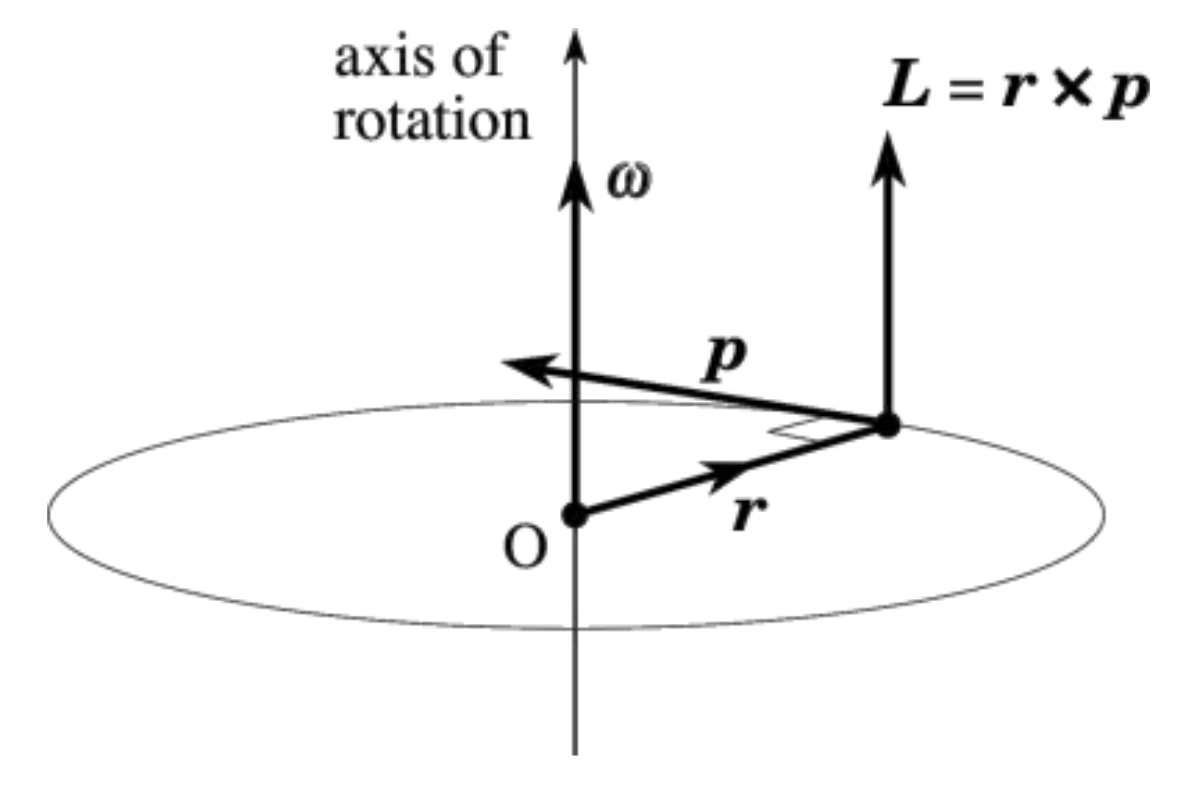
\includegraphics[width=0.5\textwidth]{images/classical_angular_momentum.png}
  \caption{Classical orbital angular momentum}
  \label{fig:classical_angular_momentum}
\end{wrapfigure}

In classical mechanics, the angular momentum of a particle relative to some axis is defined as:

\begin{equation}
    \vec{L} = \vec{r} \times \vec{p}
\end{equation}

where $\vec{r}$ is the position vector of the particle with respect to a point on the axis of rotation and $\vec{p}$ is its momentum. 

The total angular momentum of a system of particles is the sum of angular momenta of the individual particles:
\begin{equation}
    \vec{L}_\text{total} = \sum_i \vec{r}_i \times \vec{p}_i
\end{equation}

The total angular momentum varies in time according to the net external torque, which we can obtain by differentiating the total angular momentum with respect to time:
\begin{equation}
    \vec{\tau}_\text{total} = \sum_i \vec{\tau}_{\text{ext},i} = \frac{d\vec{L}_\text{total}}{dt}
\end{equation}

It follows that the total angular momentum of a system is conserved if the resultant external torque acting on the system is zero.

\subsubsection{Orbital angular momentum in quantum mechanics}

As discussed in \textbf{Section \ref{observables_and_operators}}, to obtain the quantum mechanical operator for orbital angular momentum from its classical definition, we can apply quantisation to the classical expression provided in the previous section:
\begin{equation}
    \vec{L} = \vec{R} \times \vec{P} = -i\hbar \vec{R}\times \vec{\nabla}
\end{equation}

For a system of (spin-less) particles, the total angular momentum is defined as:
\begin{equation}
    \vec{L}_\text{total} = \sum_i \vec{R}_i \times \vec{P}_i
\end{equation}

The different cartesian components of the angular momentum operator are:
\begin{equation} \label{orbital_angular_momentum_operators}
    \begin{split}
        L_x &= YP_z - ZP_y = -i\hbar \left(Y\frac{\partial}{\partial z} - Z\frac{\partial}{\partial y}\right) \\
        L_y &= ZP_x - XP_z = -i\hbar \left(Z\frac{\partial}{\partial x} - X\frac{\partial}{\partial z}\right) \\
        L_z &= XP_y - YP_x = -i\hbar \left(X\frac{\partial}{\partial y} - Y\frac{\partial}{\partial x}\right)
    \end{split}
\end{equation}
We can also define the square of the angular momentum operator:
\begin{equation}
    L^2 = L_x^2 + L_y^2 + L_z^2
\end{equation}
As expected from operators corresponding to observables, all angular momentum operators are Hermitian.

\subsubsection{Commutation relations}

The commutation relations for the orbital angular momentum operators are:
\begin{equation}
    \begin{split}
        [L_x, L_y] &= L_xL_y - L_yL_x = i\hbar L_z \\
        [L_y, L_z] &= L_yL_z - L_zL_y = i\hbar L_x \\
        [L_z, L_x] &= L_zL_x - L_xL_z = i\hbar L_y
    \end{split}
\end{equation}

\subsection{General formalism of angular momentum}

We have just defined the orbital angular momentum. However there exists a more general formalism of angular momentum, which is the \textit{total} angular momentum. Its corresponding operator is $\vec{J}$. In the case that the only contribution to the \textit{total} angular momentum is the \textit{orbital} angular momentum, then $\vec{J} = \vec{L}$. Thus, all we will see in this section can be identically applied to orbital angular momentum\footnote{In general, the total angular momentum is the sum of the \textit{orbital} angular momentum and the \textit{spin} angular momentum. The spin angular momentum is a purely quantum mechanical phenomenon, which we will discuss in \textbf{Section \ref{spin}}.}.

$\vec{J}\,^2$ is defined by its three components that satisfy:
\begin{equation} \label{eq:commutation_relations_angular_momentum}
    \begin{split}
        [J_x, J_y] &= i\hbar J_z \\
        [J_y, J_z] &= i\hbar J_x \\
        [J_z, J_x] &= i\hbar J_y
    \end{split}\qquad \vec{J}\,^2 = J_x^2 + J_y^2 + J_z^2\qquad [\vec{J}\,^2, J_k] = 0\quad (k = x, y, z)
\end{equation}

Thanks to these commutation relations, we know that we cannot measure the three components of the total angular momentum simultaneously. However, we \textit{can} simultaneously measure the total angular momentum squared $J^2$ and one of its components. There is possibility to find simultaneous eigenstates of $J^2$ and any component of $J$. However, we can only choose one component of $J$ to be measured simultaneously with $J^2$. By convention, we choose $J_z$, so that we work with a basis of eigenvectors that is common to $J^2$ and $J_z$ in all our calculations\footnote{Note that this is just a convention. There is \textit{nothing} special about the $z$ direction compared to $x$ and $y$.}.

\textit{Eigenstates of the total angular momentum operators}

Let us now look for the joint eigenstates of $J^2$ and $J_z$ and their corresponding eigenvalues. Denoting the joint eigenstates by $\ket{\alpha, \beta}$, and the corresponding eigenvalues of $J^2$ and $J_z$ by $\hbar^2\alpha$ and $\hbar \beta$, respectively, we have:
\begin{equation} \label{eq:angular_momentum_eigenstates}
    \begin{split}
        J^2\ket{\alpha, \beta} &= \hbar^2\alpha\ket{\alpha, \beta} \\
        J_z\ket{\alpha, \beta} &= \hbar\beta\ket{\alpha, \beta}
    \end{split}
\end{equation}
The factor $\hbar$ is introduced so that $\alpha$ and $\beta$ are dimensionless. We also assume that the eigenstates are orthonormal.

Now we need to introduce \textit{raising} and \textit{lowering} operators $J_+$ and $J_-$, respectively, which are defined as:
\begin{equation}
    J_\pm = J_x \pm iJ_y
\end{equation}
This leads to:
\begin{equation} \label{eq:jx_and_jy_in_terms_of_jp_and_jm}
    J_x = \frac12(J_+ + J_-)\qquad J_y = \frac{1}{2i}(J_+ - J_-)
\end{equation}
hence:
\begin{equation}
    J_x^2 = \frac14(J_+^2+J_+J_-+J_-J_++J_-^2)\qquad J_y^2 = -\frac{1}{4}(J_+^2-J_+J_--J_-J_++J_-^2)
\end{equation}
Using the commutation relations from \textbf{Equation \ref{eq:commutation_relations_angular_momentum}}, we can easily obtain:
\begin{equation} \label{eq:commutation_relations_angular_momentum_2}
    [\vec{J}\,^2, J_\pm] = 0\qquad [J_+, J_-] = 2\hbar J_z \qquad [J_z, J_\pm] = \pm\hbar J_\pm
\end{equation}
And also:
\begin{equation} \label{j_p_and_j_m_products}
    \begin{split}
        J_+J_- = J_x^2 + J_y^2 + \hbar J_z = \vec{J}\,^2 - J_z^2 + \hbar J_z\\
        J_-J_+ = J_x^2 + J_y^2 - \hbar J_z = \vec{J}\,^2 - J_z^2 - \hbar J_z
    \end{split} 
\end{equation}
These relations lead to:
\begin{equation}
    \vec{J}\,^2 = J_\pm J_\mp + J_z^2 \mp \hbar J_z = \frac12(J_+ J_- + J_- J_+) + J_z^2
\end{equation}

Since $J_\pm$ do not commute with $J_z$, the kets $\ket{\alpha, \beta}$ are not eigenstates of $J_\pm$. Using the expressions in \textbf{Equation \ref{eq:commutation_relations_angular_momentum_2}}, we can obtain:
\begin{equation} \label{eq:jz_jpm_eigenstates}
    \begin{split}
        J_z(J_\pm\ket{\alpha, \beta}) &= (J_\pm J_z \pm \hbar J_\pm)\ket{\alpha, \beta} = J_\pm J_z \ket{\alpha, \beta} \pm \hbar J_\pm \ket{\alpha, \beta} = \\
        &= \hbar \beta J_\pm \ket{\alpha, \beta} \pm \hbar J_\pm \ket{\alpha, \beta} = \hbar(\beta \pm 1)(J_\pm\ket{\alpha, \beta})
    \end{split}
\end{equation} 
hence the ket $J_\pm\ket{\alpha, \beta}$ is an eigenstate of $J_z$ with eigenvalue $\hbar(\beta \pm 1)$. Since $\vec{J}\,^2$ commutes with $J_z$, $J_\pm\ket{\alpha, \beta}$ is also an eigenstate of $\vec{J}\,^2$. Using \textbf{Equation \ref{eq:commutation_relations_angular_momentum_2}} again, which tells us that $\vec{J}\,^2$ commutes with $J_\pm$, we can determine the eigenvalue, which is $\hbar^2\alpha$:
\begin{equation} \label{eq:j2_jpm_eigenstates}
    \vec{J}\,^2(J_\pm\ket{\alpha, \beta}) = J_\pm \vec{J}\,^2\ket{\alpha, \beta} = J_\pm \hbar^2\alpha \ket{\alpha, \beta} = \hbar^2\alpha(J_\pm \ket{\alpha, \beta})
\end{equation}

If we rewrite \textbf{Equation \ref{eq:jz_jpm_eigenstates}} and \textbf{Equation \ref{eq:j2_jpm_eigenstates}} in terms of $\ket{\alpha',\beta'} = J_\pm \ket{\alpha,\beta}$:
\begin{equation}
    \begin{split}
        J_z\ket{\alpha', \beta'} &= \hbar(\beta \pm 1)\ket{\alpha', \beta'} \\
        \vec{J}\,^2\ket{\alpha', \beta'} &= \hbar^2\alpha\ket{\alpha', \beta'}
    \end{split}
\end{equation}

and if we compare with \textbf{Equation \ref{eq:angular_momentum_eigenstates}}, we can infer that $\alpha' = \alpha$ and $\beta' = \beta \pm 1$. In other words, the ket $J_\pm\ket{\alpha,\beta}$ is proportional to $\ket{\alpha, \beta\pm 1}$ (any eigenket multiplied by a constant is also an eigenket, although it may not be normalised), and we can write:
\begin{equation} \label{eq:j_p_and_j_m_eigenstates}
    J_\pm\ket{\alpha, \beta} = C_{\alpha\beta}^\pm\ket{\alpha, \beta\pm 1}
\end{equation}

So, when the operators $J_\pm$ act on a ket $\ket{\alpha, \beta}$, they do not change the first quantum number $\alpha$, but they increase (or decrease) the second quantum number $\beta$ by one unit. Hence the names \textit{raising} and \textit{lowering} operators.

Note that, for a given eigenvalue $\alpha$ of $\vec{J}\,^2$, there exists an upper limit for the \textit{absolute value}\footnote{That is to say, $\beta$ is bounded from above \textit{and} below.} of the quantum number $\beta$. This is due to the fact that the operator $\vec{J}\,^2 - J_z^2$ is positive definite, as the matrix elements of $\vec{J}\,^2 - J_z^2 = J_x^2 + J_y^2 \geq 0$ are non-negative, so we can write:
\begin{equation}
    \braket{\alpha, \beta| \vec{J}\,^2 - J_z^2 | \alpha, \beta} = \hbar^2(\alpha - \beta^2) \geq 0\quad \Longrightarrow\quad \alpha \geq\beta^2
\end{equation} 

Since $\beta$ has an upper limit, $\beta_\text{max}$, there must exist a state $\ket{\alpha, \beta_\text{max}}$ which cannot be raised further:
\begin{equation}
    J_+\ket{\alpha, \beta_\text{max}} = 0
\end{equation}

Using this, along with \textbf{Equation \ref{j_p_and_j_m_products}}, we can obtain:
\begin{equation}
    J_-J_+\ket{\alpha,\beta_\text{max}} = (\vec{J}\,^2 - J_z^2 - \hbar J_z)\ket{\alpha,\beta_\text{max}} = \hbar^2(\alpha-\beta_\text{max}^2 - \beta_\text{max})\ket{\alpha,\beta_\text{max}} = 0
\end{equation}
hence:
\begin{equation}
    \alpha = \beta_\text{max}(\beta_\text{max} + 1)
\end{equation}

Since $\beta$ has a lower limit, $\beta_\text{min}$, there must exist a state $\ket{\alpha, \beta_\text{min}}$ which cannot be lowered further, which we reach after $n$ successive applications of $J_-$ on $\ket{\alpha, \beta_\text{max}}$:
\begin{equation} \label{eq:alpha_beta_max}
    J_-\ket{\alpha, \beta_\text{min}} = 0
\end{equation}

Using this, along with \textbf{Equation \ref{j_p_and_j_m_products}}, we can obtain:
\begin{equation}
    J_+J_-\ket{\alpha,\beta_\text{min}} = (\vec{J}\,^2 - J_z^2 + \hbar J_z)\ket{\alpha,\beta_\text{min}} = \hbar^2(\alpha-\beta_\text{min}^2 + \beta_\text{min})\ket{\alpha,\beta_\text{min}} = 0
\end{equation}
hence:
\begin{equation} \label{eq:alpha_beta_min}
    \alpha = \beta_\text{min}(\beta_\text{min} - 1)
\end{equation}

Comparing \textbf{Equation \ref{eq:alpha_beta_max}} and \textbf{Equation \ref{eq:alpha_beta_min}}, we can infer that:
\begin{equation}
    \beta_\text{max} = -\beta_\text{min}
\end{equation}

Since $\beta_\text{min}$ was reached after $n$ successive applications of $J_-$ on $\ket{\alpha, \beta_\text{max}}$, it follows that:
\begin{equation}
    \beta_\text{max} = \beta_\text{min} + n, \qquad n\in \N
\end{equation}

Combining the last two equations, we obtain:
\begin{equation}
    \beta_\text{min} = -\frac{n}{2}\qquad \beta_\text{max} = \frac{n}{2}
\end{equation}

Which means that $\beta_\text{max}$ is either an integer or a half-odd-integer. We can now introduce the notation:
\begin{equation}
    j = \beta_\text{max} = \frac{n}{2}\qquad m = \beta
\end{equation}
hence, we can express $\alpha$ as:
\begin{equation}
    \alpha = j(j+1)
\end{equation}
And we can infer that the values of $m$ lie between $-j$ and $j$:
\begin{equation}
    -j \leq m \leq j
\end{equation}

We can now summarise the results we have obtained so far:
\begin{definition}
    The eigenvalues of $\vec{J}\,^2$ and $J_z$ corresponding to the joint eigenvectors $\ket{j,m}$ are given, respectively, by $\hbar^2j(j+1)$ and $\hbar m$:
    \begin{equation}
        \vec{J}\,^2\ket{j,m} = \hbar^2j(j+1)\ket{j,m}\qquad J_z\ket{j,m} = \hbar m\ket{j,m}
    \end{equation}
    where $j = 0,\, 1/2,\, 1,\, 3/2,\, ...$ and $m = -j, -(j-1), \dots, j-1, j$. We see that the spectra of the angular momentum operators $\vec{J}\,^2$ and $J_z$ are discrete. Since the eigenstates corresponding to different angular momenta are orthogonal, and since the angular momentum spectra are discrete, the orthonormality condition is:
    \begin{equation}
        \braket{j',m'|j,m} = \delta_{j',j}\delta_{m',m}
    \end{equation}
\end{definition}

Let us now determine the normalisation constant $C_{\alpha\beta}^\pm$ in \textbf{Equation \ref{eq:j_p_and_j_m_eigenstates}}, which we can rewrite in terms of $j$ and $m$ as:
\begin{equation}
    J_\pm\ket{j,m} = C_{jm}^\pm\ket{j,m\pm 1}
\end{equation}
Since $\ket{j,m+1}$ is normalised:
\begin{equation}
    (J_+\ket{j,m})^\dagger (J_+\ket{j,m}) = |C_{jm}^+|^2\braket{j, m+1|j, m+1} = |C_{jm}^+|^2
\end{equation}

Since $J_+ = J_x + iJ_y$ and the operators $J_x$ and $J_y$ are Hermitian, we have:
\begin{equation}
    J_+^\dagger = (J_x+iJ_y)^\dagger = J_x^\dagger -iJ_y^\dagger = J_x - iJ_y = J_-
\end{equation}
So we can also write:
\begin{equation}
    \braket{j,m|J_-J_+|j,m} = \braket{j,m|J_+^\dagger J_+|j,m} = (J_+\ket{j,m})^\dagger (J_+\ket{j,m}) = |C_{jm}^+|^2
\end{equation}

But since $J_-J_+ = \vec{J}\,^2 - J_z^2 - \hbar J_z$ and $\ket{j,m}$ is orthonormal, we can also write:

\begin{equation}
    \begin{split}
        |C_{jm}^+|^2 &= \braket{j,m|J_-J_+|j,m} = \braket{j,m|\vec{J}\,^2 - J_z^2 - \hbar J_z|j,m} = \\
        &= \braket{j,m|\vec{J}\,^2|j,m} - \braket{j,m|J_z^2|j,m} - \hbar\braket{j,m|J_z|j,m} = \\
        &= \braket{j,m|\hbar^2j(j+1)|j,m} - \braket{j,m|\hbar^2m^2|j,m} - \hbar\braket{j,m|\hbar m|j,m} = \\
        &= \hbar^2j(j+1)\braket{j,m|j,m} - \hbar^2m^2\braket{j,m|j,m} - \hbar^2m\braket{j,m|j,m} = \\
        &= \hbar^2j(j+1) - \hbar^2m^2 - \hbar^2m = \\
        &= \hbar^2(j(j+1)-m(m+1))
    \end{split}
\end{equation}

So we conclude that\footnote{Note that here we would actually have to add a phase factor $e^{i\theta}$ so that $C_{jm}^+ = \hbar \sqrt{j(j+1)-m(m+1)}e^{i\theta}$. This is beacuse $C_{jm}^+$ is, in general terms, a complex number. As we have the freedom of choice, we take $C_{jm}^+$ to be real and positive. The same argument applies to $C_{jm}^-$.}:
\begin{equation}
    C_{jm}^+ = \hbar \sqrt{j(j+1)-m(m+1)}
\end{equation}

Similarly, we can obtain:
\begin{equation}
    C_{jm}^- = \hbar \sqrt{j(j+1)-m(m-1)}
\end{equation}

So, we now have the raising and lowering operators completely defined:
\begin{definition}
    The raising and lowering operators $J_+$ and $J_-$ are given by:
    \begin{equation}
        J_\pm = J_x \pm iJ_y
    \end{equation}
    Their action on a ket $\ket{j,m}$ raises or lowers the second quantum number $m$ by one unit, respectively:
    \begin{equation} \label{eq:raising_and_lowering_operators_J}
        J_\pm\ket{j,m} = \hbar \sqrt{j(j+1)-m(m\pm1)}\ket{j,m\pm 1}
    \end{equation}
\end{definition}

\subsubsection{Matrix representation of angular momentum}

The formalism we discussed in the previous section is completely general and independent on the choice of representation. There are many ways to represent the angular momentum operators and their eigenstates, and in this section we will discuss the matrix representation of angular momentum, where eigenkets and operators are represented by column and square matrices, respectively.

Since $\vec{J}\,^2$ and $J_z$ commute, the set of their common eigenstates $\{\ket{j, m}\}$ can be chosen as a basis. This basis is discrete, orthonormal and complete. The orthonormality condition and the completeness relation can be expressed, respectively, as:
\begin{equation}
    \braket{j',m'|j,m} = \delta_{j',j}\delta_{m',m} \qquad\sum_{j}\sum_{m=-j}^{j}\ket{j,m}\bra{j,m} = \Imat
\end{equation}
The matrix elements of the $\vec{J}\,^2$ and $J_z$ operators in this basis are:
\begin{equation}
    \begin{split}
        \bra{j',m'}\vec{J}\,^2\ket{j,m} &= \hbar^2j(j+1)\delta_{j',j}\delta_{m',m} \\
        \bra{j',m'}J_z\ket{j,m} &= \hbar m\delta_{j',j}\delta_{m',m}
    \end{split}
\end{equation}
Clearly, $\vec{J}\,^2$ and $J_z$ are diagonal in this basis, their diagonal elements being $\hbar^2j(j+1)$ and $\hbar m$, respectively. However, as $J_\pm$ do not commute with $\vec{J}\,^2$ and $J_z$, they are not diagonal in this basis. Their matrix elements are:
\begin{equation}
    \bra{j',m'}J_\pm\ket{j,m} = \hbar \sqrt{j(j+1)-m(m\pm 1)}\delta_{j',j}\delta_{m',m\pm 1} \\
\end{equation}
The matrices of $J_x$ and $J_y$ are obtained by adding and subtracting the matrices of $J_+$ and $J_-$, respectively, as seen in \textbf{Equation \ref{eq:jx_and_jy_in_terms_of_jp_and_jm}}:
\begin{equation}
    J_x = \frac12(J_+ + J_-)\qquad J_y = \frac{1}{2i}(J_+ - J_-)
\end{equation}

\subsubsection{Geometrical representation of angular momentum}

The expected value of the angular momentum operator for a state $\ket{j,m}$, denoted as $\braket{\vec{J}}$, is given by:
\begin{equation}
    \braket{\vec{J}} = \sqrt{\braket{\vec{J}\,^2}} = \sqrt{\braket{j,m|\vec{J}\,^2|j,m}} = \hbar\sqrt{j(j+1)}
\end{equation}
with $z$-component given by: 
\begin{equation}
    \braket{J_z} = \braket{j,m|J_z|j,m} = \hbar m
\end{equation}

Recalling that $J_x^2 + J_y^2 = \vec{J}\,^2 - J_z^2$, we can also give the component of the angular momentum that lies in the $xy$-plane as:
\begin{equation}
    \braket{J_{xy}} = \sqrt{\braket{J_x^2 + J_y^2}} = \sqrt{\braket{\vec{J}\,^2 - J_z^2}} = \hbar\sqrt{j(j+1) - m^2}
\end{equation}

As expected, it is verified that:
\begin{equation}
    \braket{J_{xy}}^2 + \braket{J_z}^2 = \left(\hbar \sqrt{j(j+1)-m^2}\right)^2+(\hbar m)^2 = \hbar^2j(j+1) = \braket{\vec{J}\,}^2
\end{equation}   

Graphically, we can show this with a diagram like the one on \textbf{Figure \ref{fig:angular_momentum_diagram}}, which shows the graphical representation of the angular momentum $j=2$ for the state $\ket{j,m} = \ket{2,m}$ with $m = -2, -1, 0, 1, 2$. 

\begin{figure}[htbp]
    \centering
    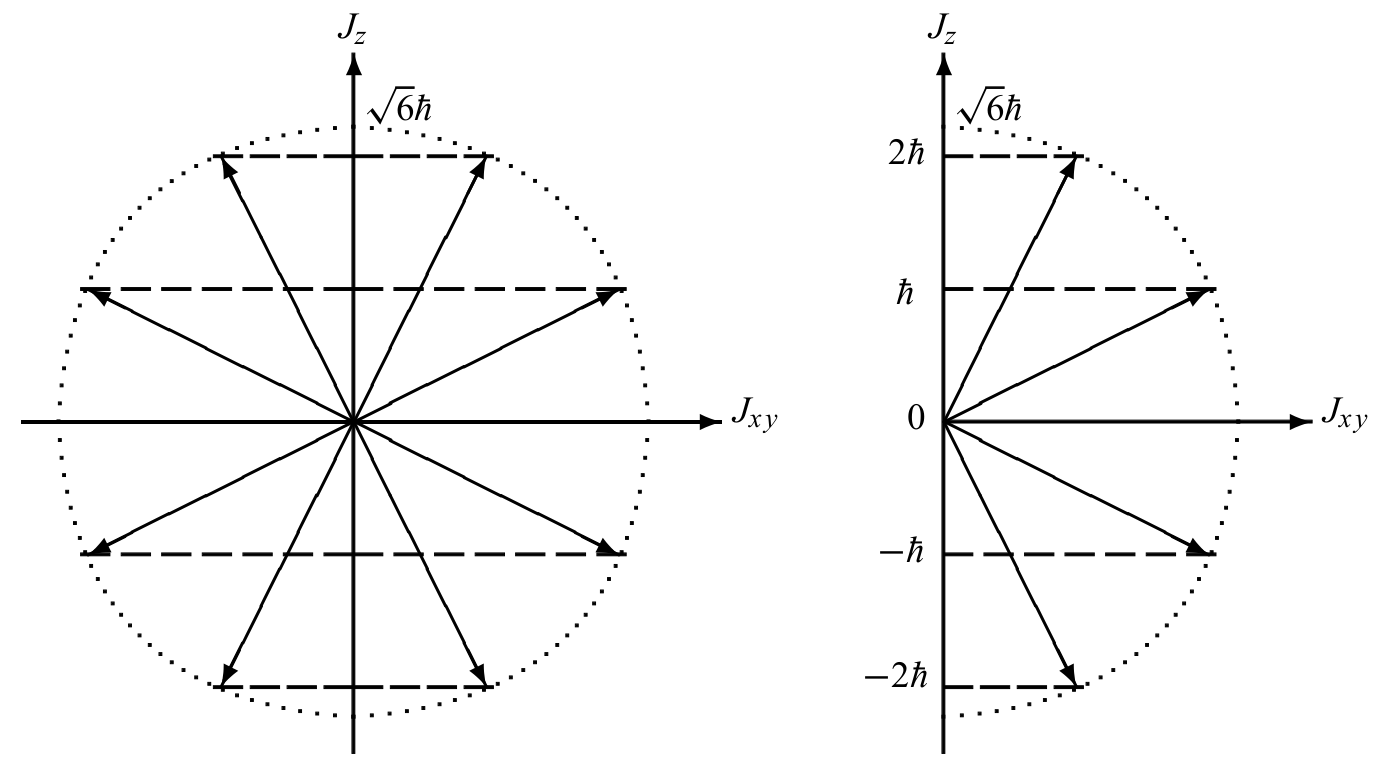
\includegraphics[width=0.8\textwidth]{images/graphical_angular_momentum.png}
    \caption{Graphical representation of the angular momentum $j = 2$ for the state $\ket{j,m} = \ket{2,m}$ with $m = -2, -1, 0, 1, 2$. The radius of the circle is $\hbar\sqrt{j(j+1)} = \hbar \sqrt{6}$.}
    \label{fig:angular_momentum_diagram}
\end{figure}

In the classical sense, we can think of $\vec{J}\,^2$ as a vector whose endpoint lies on a sphere of radius $\hbar\sqrt{j(j+1)}$, rotating about the $z$-axis along the surface of a cone, and whose projection on the $z$-axis has length $\hbar m$. The angle $\theta$ between the $z$-axis and the vector $\vec{J}\,^2$ is given by:
\begin{equation}
    \cos\theta = \frac{\braket{J_z}}{\braket{\vec{J}\,}} = \frac{\hbar m}{\hbar\sqrt{j(j+1)}} = \frac{m}{\sqrt{j(j+1)}}
\end{equation}
Notice that, as the values of the quantum number $m$ are limited to $-j, -(j-1), ..., j-1, j$, the angle $\theta$ is also limited to a discrete set of $2j+1$ values.

Since all the orientations of $\vec{J}\,^2$ on the surface of the cone are equaly likely, the projection of $\vec{J}\,^2$ on both the $x$-axes and $y$-axes averages out to zero. This can also be demostrated mathematically by calculating the expected values of $J_x$ and $J_y$ using \textbf{Equation \ref{eq:jx_and_jy_in_terms_of_jp_and_jm}}:
\begin{equation}
    \begin{split}
        \braket{J_x} &= \braket{j,m|J_x|j,m} = \frac12\braket{j,m|(J_+ + J_-)|j,m} = \frac12\braket{j,m|J_+|j,m} + \frac12\braket{j,m|J_-|j,m} = \\
        &= \frac{\hbar}{2}\sqrt{j(j+1)-m(m+1)}\braket{j,m|j,m+1} + \frac{\hbar}{2}\sqrt{j(j+1)-m(m-1)}\braket{j,m|j,m-1} = 0
    \end{split}
\end{equation}
\begin{equation}
    \begin{split}
        \braket{J_y} &= \braket{j,m|J_y|j,m} = \frac{1}{2i}\braket{j,m|(J_+ - J_-)|j,m} = \frac{1}{2i}\braket{j,m|J_+|j,m} - \frac{1}{2i}\braket{j,m|J_-|j,m} = \\
        &= \frac{\hbar}{2i}\sqrt{j(j+1)-m(m+1)}\braket{j,m|j,m+1} - \frac{\hbar}{2i}\sqrt{j(j+1)-m(m-1)}\braket{j,m|j,m-1} = 0
    \end{split}
\end{equation}

\subsection{Position representation of orbital angular momentum}

As we already saw in a previous section, in the position representation, the orbital angular momentum operators are given in cartesian coordinates by \textbf{Equation \ref{orbital_angular_momentum_operators}}. However, it is more convenient to work in spherical (or polar) coordinates, since, as we shall see, the various angular momentum operators act only on the angular variables and and not on the $r$ variable. We can rewrite the angular momentum operators in spherical coordinates as:

\begin{equation} \label{LxLyLz}
    \begin{split}
        L_x &= i\hbar \left(\sin\phi\frac{\partial}{\partial\theta} + \frac{\cos\phi}{\tan\theta}\frac{\partial}{\partial\phi}\right) \\
        L_y &= i\hbar \left(-\cos\phi\frac{\partial}{\partial\theta} + \frac{\sin\phi}{\tan\theta}\frac{\partial}{\partial\phi}\right) \\
        L_z &= -i\hbar \frac{\partial}{\partial\phi}
    \end{split}
\end{equation}

We can also rewrite the $L_\pm$ and $L^2$ operators in spherical coordinates:
\begin{equation}
    \begin{split}
        L_\pm &= \pm\hbar e^{\pm i\phi}\left(\frac{\partial}{\partial\theta} \pm i\cot\theta\frac{\partial}{\partial\phi}\right) \\
        \vec{L}\,^2 &= -\hbar^2\left[\frac{\partial^2}{\partial \theta^2}+ \frac{1}{\tan \theta} \frac{\partial }{\partial \theta } + \frac{1}{\sin^2\theta}\frac{\partial^2}{\partial \phi^2}\right]
    \end{split}
\end{equation}

Then, the original eigenproblem for a spinless particle can be written as:
\begin{equation} 
    \begin{split}
        \vec{L}\,^2\ket{l,m} &= \hbar^2l(l+1)\ket{l,m} \\
        L_z\ket{l,m} &= \hbar m\ket{l,m}
    \end{split}
\end{equation}
can be written in the $r$-representation as:
\begin{equation} 
    \begin{split}
        \vec{L}\,^2\psi_{l,m} (r, \theta, \phi) &= \hbar^2l(l+1)\psi_{l,m} (r, \theta, \phi) \\
        L_z\psi_{l,m} (r, \theta, \phi) &= \hbar m\psi_{l,m} (r, \theta, \phi)
    \end{split}
\end{equation}
where, as the operators act only on the angular variables, the eigenfunctions are separable:
\begin{equation}
    \psi_{l,m} (r, \theta, \phi) = R_{l}(r)Y_l^m(\theta, \phi)
\end{equation}

The solution to the angular part of this eigenproblem are \textbf{spherical harmonics}:
\begin{equation}
    \begin{split}
        Y_l^m(\theta, \phi) &= \varepsilon\sqrt{\frac{(2l+1)}{4\pi}\frac{(l-|m|)!}{(l+|m|)!}}P_l^m(\cos\theta)e^{im\phi} \\
        \varepsilon &= \begin{cases}
            (-1)^m & \text{if } m \geq 0 \\
            1 & \text{if } m < 0
        \end{cases}
    \end{split}
\end{equation}

where $P_l^m(\cos\theta)$ are the \textbf{associated Legendre polynomials}, which are given by:
\begin{equation}
    P_l^m(x) = (1-x^2)^{|m|/2}\frac{d^{|m|}}{dx^{|m|}}P_l(x), \qquad P_l(x) = \frac{1}{2^ll!}\frac{d^l}{dx^l}(x^2-1)^l
\end{equation}

Spherical harmonics are joint eigenfunctions of the operators $\vec{L}\,^2$ and $L_z$, as both these operators commute. We can therefore write:
\begin{equation} \label{spherical_eig_eqn}
    \begin{split}
        \vec{L}\,^2Y_l^m(\theta, \phi) &= \hbar^2l(l+1)Y_l^m(\theta, \phi) \\
        L_zY_l^m(\theta, \phi) &= \hbar mY_l^m(\theta, \phi)
    \end{split}
\end{equation}


They are also functions with a well-defined parity, as they are eigenfunctions of the parity operator $P$:
\begin{equation} \label{parity_spherical_harmonics}
    PY_l^m(\theta, \phi) = Y_l^m(\pi-\theta, \pi+\phi) = (-1)^lY_l^m(\theta, \phi)
\end{equation}

Also, the complex conjugate of a spherical harmonic is given by:
\begin{equation}
    \left[Y_l^{m}(\theta, \phi)\right]^* = (-1)^mY_l^{-m}(\theta, \phi)
\end{equation}

\subsubsection{Values of $m$ and $l$}

Using $L_z = -i\hbar \partial /\partial\phi$ (from \textbf{Equation \ref{LxLyLz}}), we can rewrite \textbf{Equation \ref{spherical_eig_eqn}} as:
\begin{equation}
    -i\hbar \frac{\partial}{\partial\phi}Y_l^m(\theta, \phi) = \hbar mY_l^m(\theta, \phi)
\end{equation}

From this, we obtain that $Y_l^m(\theta, \phi) = F_l^m(\theta) e^{im\phi}$. However, as wave functions must be continuous at all points in space, we must impose that:
\begin{equation}
    Y_l^m(\theta, \phi=0) = Y_l^m(\theta, \phi=2\pi) \longrightarrow 1 = e^{2\pi mi}
\end{equation}
We already had from the general formalism of angular momentum that $m$ had to be either integral or half-integral. Now, we have this additional condition that restricts $m$ to being strictly integer, as half-integer values of $m$ would result in $e^{2\pi mi}=-1$. But, if $m$ is integral, then $l$ must also be integral. Therefore, we can now define:

\begin{definition}
    The eigenvalues of $\vec{L}\,^2$ and $L_z$ corresponding to the joint eigenvectors $\ket{l,m}$ are given, respectively, by $\hbar^2l(l+1)$ and $\hbar m$:
    \begin{equation}
        \vec{L}\,^2\ket{l,m} = \hbar^2l(l+1)\ket{l,m}\qquad L_z\ket{l,m} = \hbar m\ket{l,m}
    \end{equation}
    where $l = 0,\, 1,\, 2,\, 3,\, ...$ and $m = -l, -(l-1), \dots, l-1, l$. We see that the spectra of the orbital angular momentum operators $\vec{L}\,^2$ and $L_z$ are discrete. Since the eigenstates corresponding to different angular momenta are orthogonal, and since the angular momentum spectra are discrete, the orthonormality condition is:
    \begin{equation}
        \braket{l',m'|l,m} = \delta_{l',l}\delta_{m',m}
    \end{equation}

    Note that the $m$ we use here is different to the one used in the general angular momentum $\vec{J}$. In order to tell them apart, this one we are using here is often denoted as $m_l$.
\end{definition}

\subsection{Spin angular momentum} \label{spin}

Spin angular momentum is one of the most fundamental properties of an electron and other elementary particles, despite the fact that it has no classical analogue, in contrast to orbital angular momentum. Its existence was discovered in 1922 by Stern and Gerlach, who observed that a beam of ground-state silver atoms, which have no orbital angular momentum, split in two when passing through a non-uniform magnetic field. This unexpected result, caused by the spin angular momentum of the $5s$ valence electron, led them to postulate the existence of a new angular momentum phenomenon different from orbital angular momentum, and they called it \textbf{spin}. The theory of spin is identical to the general theory of angular momentum and, by analogy with the vector $\vec{J}$, the spin is also represented by a vector operator $\vec{S}$.

From the classical theory of electromagnetism, an orbital magnetic dipole moment is generated with the orbital motion of a particle of charge $q$:
\begin{equation} \label{orbital_magnetic_dipole_moment}
    \vec{\mu}_L = \frac{q}{2m}\vec{L}
\end{equation}
where $\vec{L}$ is the orbital angular momentum of the particle, $m$ its mass, and $c$ the speed of light. Similarly, if we follow a classical analysis, we can define the \textbf{spin magnetic dipole moment} of a particle as:
\begin{equation} \label{spin_magnetic_dipole_moment_pre}
    \vec{\mu}_S = \frac{q}{2m}\vec{S}
\end{equation}

Although this expression cannot be derived classically, as there is no classical equivalent of spin, it can still be postulated by analogy to the orbital magnetic dipole moment. However, there is one correction that we need to make to \textbf{Equation \ref{spin_magnetic_dipole_moment_pre}}: it turns out that, for the electron, the orbital magnetic dipole moment is actually twice its classical expression. For other particles, this ratio, which we call gyromagnetic ratio (or Landé factor) $g_s$, can vary. Taking this effect into account, we obtain\footnote{The ratio $g_s$ can be obtained using Dirac's relativistic quantum theory. For the electron, $g_s = 2$.}:
\begin{equation} \label{spin_magnetic_dipole_moment}
    \vec{\mu}_S = g_s\frac{q}{2m}\vec{S}
\end{equation}

When the electron is placed in a magnetic field $\vec{B}$ and if the field is inhomogeneous, a force will be exerted on the electron's intrinsic dipole moment; the direction and magnitude of the force depend on the relative orientation of the field and the dipole. This force tends to align $\vec{\mu}_S$  along $\vec{b}$, producing a precessional motion of $\vec{\mu}_S$ around $\vec{b}$.



\subsubsection{Quantum description of spin}

Until now, we have studied the quantisation of \textit{orbital variables}. With the position $\vec{r}$ and the momentum $\vec{p}$ of a particle such as the electron, we associated the observables $\vec{R}$ and $\vec{P}$ acting in the state space $\varepsilon_{\vec{r}}$, which is isomorphic to the space $\F$ of wave functions. All physical quantities are functions of the fundamental variables $\vec{r}$ and $\vec{p}$, and the quantisation rules enable us to associate with them observables acting in $\vec{r}$. We shall call $\varepsilon_{\vec{r}}$ the \textit{orbital state space}.

To these \textit{orbital variables} we have studied up until now, we will add the \textit{spin variables}, which satisfy the following postulates:

\begin{postulate}
    \textbf{The spin operator:} The spin operator $\vec{S}$ is an angular momentum vector operator whose components $S_x$, $S_y$ and $S_z$ satisfy the commutation relations of angular momentum operators:
    \begin{equation}
        [S_x, S_y] = i\hbar S_z, \qquad [S_y, S_z] = i\hbar S_x, \qquad [S_z, S_x] = i\hbar S_y
    \end{equation}
\end{postulate}

\begin{postulate}
    \textbf{Spin state space:} The spin operators act in a new space, the ``spin state space'' $\varepsilon_s$, where $\vec{S}\,^2$ and $S_z$ constitute a CSCO. The space $\varepsilon_s$ is thus spanned by the set of eigenstates $\ket{s,m_s}$ common to $\vec{S}\,^2$ and $S_z$:
    \begin{equation} \label{eigenstates_of_S2_and_Sz}
        \vec{S}\,^2 \ket{s, m_s} = \hbar^2s(s+1)\ket{s, m_s}, \qquad S_z \ket{s, m_s} = \hbar m_s\ket{s, m_s}
    \end{equation}
    where $s = 0,\, 1/2,\, 1,\, 3/2,\, ...$ and $m_s = -s, -(s-1), ..., s-1, s$. A given particle is characterised by a \textit{unique}, \textit{specific} and \textit{immutable} value\footnote{For example, the electron has $s = 1/2$, the photon has $s = 1$, the proton has $s = 1/2$, the neutron has $s = 1/2$, etc. The value of $s$ is called the \textbf{spin quantum number}.} of $s$: this particle is said to have a spin $s$. The spin state space $\varepsilon_s$ is therefore always of finite dimension $(2s + 1)$, and all spin states are eigenvectors of $\vec{S}\,^2$ with the same eigenvalue $s(s + 1)\hbar^2$.
    
    Similarly, we have:

    \begin{equation} \label{eq:spin_pm_ops}
        S_\pm \ket{s, m_s} = \hbar \sqrt{s(s+1)-m_s(m_s\pm 1)}\ket{s, m_s\pm 1}
    \end{equation}
    where $S_\pm = S_x \pm iS_y$, and:
    \begin{equation}
        \braket{S_x^2} = \braket{S_y^2} = \frac{\hbar^2}{2}\left[s(s+1) - m_s^2\right]
    \end{equation}

    The spin states form an orthonormal and complete basis:
    \begin{equation}
        \braket{s', m_s'|s, m_s} = \delta_{s',s}\delta_{m_s',m_s} \qquad \sum_s\sum_{m_s=-s}^{s}\ket{s,m_s}\bra{s,m_s} = \Imat
    \end{equation}
\end{postulate}

\begin{postulate} \label{postulate:tensor_product}
    \textbf{The state space:} The state space $\varepsilon$ of a particle is the tensor product of the orbital state space $\varepsilon_{\vec{r}}$ and the spin state space $\varepsilon_s$:
    \begin{equation}
        \varepsilon = \varepsilon_{\vec{r}} \otimes \varepsilon_s
    \end{equation}
\end{postulate}

Note that the spin angular momentum is an \textbf{intrinsic property of the particle}. It has nothing to do with motion of the particle in space. All angular momentum related to the spatial dependence of the wave function is included in $\vec{L}$. Therefore, spin angular momentum cannot be described by any function of the position variables. An important consequence of \textbf{Postulate \ref{postulate:tensor_product}} related to this is that all \textit{orbital observables} commute with all \textit{spin observables}, as they act on different state spaces. Spin operators act on the spin part and leave the spatial part unchanged, and vice versa. In other words, the spin of a particle and its orbital motion do not affect each other. 

\subsubsection{Spin 1/2}

In the case of a particle of spin $s=1/2$, the spin state $\varepsilon_s$ is two-dimensional, as we have two possible values of $m_s = \pm 1/2$. In this space, we will consider the orthonormal basis of eigenstates common to $\vec{S}\,^2$ and $S_z$:
\begin{itemize}
    \item For $s=1/2$ and $m_s=1/2$, we have $\ket{1/2, 1/2} = \ket{\uparrow}=\ket{+}$
    \item For $s=1/2$ and $m_s=-1/2$, we have $\ket{1/2, -1/2} = \ket{\downarrow}=\ket{-}$
\end{itemize}

With this basis, we can write the eigenvaue equations from \textbf{Equation \ref{eigenstates_of_S2_and_Sz}} as:
\begin{equation} \label{eq:spin_1/2_eigenstates}
    \vec{S}\,^2\ket{\pm} =\frac{3}{4}\hbar^2\ket{\pm}, \qquad S_z\ket{\pm} = \pm\frac{1}{2}\hbar\ket{\pm}
\end{equation}

\textbf{Matrix representation}

Note from \textbf{Equation \ref{eq:spin_1/2_eigenstates}} that \textit{all} kets of the basis of $\varepsilon_s$ are eigenvectors of $\vec{S}\,^2$ with the same eigenvalue $3\hbar^2/4$. This causes $\vec{S}\,^2$ to be proportional to the unity operator $\Imat$ of $\varepsilon_s$:
\begin{equation}
    \vec{S}\,^2 = \frac{3}{4}\hbar^2\Imat
\end{equation}

We can also see this by taking the matrix elements of $\vec{S}\,^2$ explicitly:
\begin{equation}
    \vec{S}\,^2 = \begin{pmatrix}
        \braket{+|\vec{S}\,^2|+} & \braket{+|\vec{S}\,^2|-} \\
        \braket{-|\vec{S}\,^2|+} & \braket{-|\vec{S}\,^2|-}
    \end{pmatrix} = \begin{pmatrix}
        \frac34\hbar^2\braket{+|+} & \frac34\hbar^2\braket{+|-} \\
        \frac34\hbar^2\braket{-|+} & \frac34\hbar^2\braket{-|-}
    \end{pmatrix} =\frac{3}{4}\hbar^2\begin{pmatrix}
        1 & 0 \\
        0 & 1
    \end{pmatrix} = \frac{3}{4}\hbar^2\Imat
\end{equation}

The matrix of $S_z$ can also be obtained easily from the eigenvalue equation:
\begin{equation}
    S_z = \begin{pmatrix}
        \braket{+|S_z|+} & \braket{+|S_z|-} \\
        \braket{-|S_z|+} & \braket{-|S_z|-}
    \end{pmatrix} = \begin{pmatrix}
        \frac12\hbar\braket{+|+} & -\frac12\hbar\braket{+|-} \\
        \frac12\hbar\braket{-|+} & -\frac12\hbar\braket{-|-}
    \end{pmatrix} =\frac{\hbar}{2}\begin{pmatrix}
        1 & 0 \\
        0 & -1
    \end{pmatrix}
\end{equation}

From \textbf{Equation \ref{eq:spin_pm_ops}}, we can obtain:
\begin{equation}
    \begin{split}
        S_+\ket{+} &= 0 \\
        S_+\ket{-} &= \hbar \sqrt{\frac12\left(\frac12+1\right)-\left(-\frac12\right)\left(\left(-\frac12\right)+1\right)}\ket{+} = \hbar\ket{+} \\
        S_-\ket{+} &= \hbar \sqrt{\frac12\left(\frac12+1\right)-\frac12\left(\frac12-1\right)}\ket{-} = \hbar\ket{-} \\
        S_-\ket{-} &= 0
    \end{split}
\end{equation}

Therefore, the matrices of $S_+$ and $S_-$ are:
\begin{equation}
    S_+ = \begin{pmatrix}
        \braket{+|S_+|+} & \braket{+|S_+|-} \\
        \braket{-|S_+|+} & \braket{-|S_+|-}
    \end{pmatrix} = \begin{pmatrix}
        0 & \hbar\braket{+|+} \\
        0 & \hbar\braket{-|+}
    \end{pmatrix} = \hbar\begin{pmatrix}
        0 & 1 \\
        0 & 0
    \end{pmatrix}
\end{equation}

\begin{equation}
    S_- = \begin{pmatrix}
        \braket{+|S_-|+} & \braket{+|S_-|-} \\
        \braket{-|S_-|+} & \braket{-|S_-|-}
    \end{pmatrix} = \begin{pmatrix}
        \hbar\braket{+|-} & 0 \\
        \hbar\braket{-|-} & 0
    \end{pmatrix} = \hbar\begin{pmatrix}
        0 & 0 \\
        1 & 0
    \end{pmatrix}
\end{equation}

And since $S_x = \frac12(S_+ + S_-)$ and $S_y = \frac{1}{2i}(S_+ - S_-)$, we can obtain the matrices of $S_x$ and $S_y$:
\begin{equation}
    S_x = \frac{\hbar}{2}\begin{pmatrix}
        0 & 1 \\
        1 & 0
    \end{pmatrix}, \qquad S_y = \frac{\hbar}{2}\begin{pmatrix}
        0 & -i \\
        i & 0
    \end{pmatrix}
\end{equation}

We can express the joint eigenvectors of $\vec{S}\,^2$ and $S_z$ in terms of two-element column matrices known as \textit{spinnors}:
\begin{equation}
    \ket{+} = \begin{pmatrix}
        1 \\
        0
    \end{pmatrix}, \qquad \ket{-} = \begin{pmatrix}
        0 \\
        1
    \end{pmatrix}
\end{equation}

Any vector in the state space $\varepsilon_s$ can be written as a linear combination of the basis vectors $\ket{\pm}$:
\begin{equation}
    \ket{\psi} = c_+\ket{+} + c_-\ket{-}
\end{equation}
where $c_\pm$ are complex numbers. We can also write $\ket{\psi}$ in the form:
\begin{equation}
    \ket{\psi} = \begin{pmatrix}
        c_+ \\
        c_-
    \end{pmatrix}
\end{equation}

\textbf{Pauli matrices}

When $s=1/2$, it is convenient to introduce the \textbf{Pauli matrices}, $\sigma_x$, $\sigma_y$ and $\sigma_z$, which are defined as:
\begin{equation}
    \vec{S} = \frac{\hbar}{2}\vec{\sigma}
\end{equation}

So that:
\begin{equation}
    \frac{\hbar}{2}\sqrt{S_x^2+S_y^2+S_z^2} = \sqrt{\sigma_x^2+\sigma_y^2+\sigma_z^2}\longrightarrow \sqrt{\left(\frac{\hbar}{2}S_x\right)^2+\left(\frac{\hbar}{2}S_y\right)^2+\left(\frac{\hbar}{2}S_z\right)^2} = \sqrt{\sigma_x^2+\sigma_y^2+\sigma_z^2}\to
\end{equation}

Finally:
\begin{equation}
    \sigma_x = \frac{\hbar}{2}S_x = \begin{pmatrix}
        0 & 1 \\
        1 & 0
    \end{pmatrix}, \qquad \sigma_y = \frac{\hbar}{2}S_y = \begin{pmatrix}
        0 & -i \\
        i & 0
    \end{pmatrix}, \qquad \sigma_z = \frac{\hbar}{2}S_z = \begin{pmatrix}
        1 & 0 \\
        0 & -1
    \end{pmatrix} 
\end{equation}

\subsubsection{Spin-orbit coupling}

Spin-orbit coupling in hydrogen is an effect that arises from the interaction between the electron's spin magnetic moment, $\vec{\mu}_S$, and the proton's orbtial magnetic field $\vec{B}$.

The origin of the magnetic field experienced by the electron moving at $\vec{v}$ in a circular orbit around the proton can be explained classically as follows. The electron, within its rest frame, sees the proton moving at $-\vec{v}$ in a circular orbit around it (\textbf{Figure \ref{fig:spin_orbit_coupling}}). From classical electrodynamics, the magnetic field experienced by the electron is:
\begin{equation} \label{eq:magnetic_field}
    \vec{B} = -\frac{\vec{v}}{c^2}\times \vec{E} = -\frac{\vec{p}}{m_ec^2}\times \vec{E} = \frac{\vec{E}}{m_ec^2}\times \vec{p}
\end{equation}
where $\vec{p} = m_e\vec{v}$ is the linear momentum of the electron and $\vec{E}$ is the electric field generated by the proton, which is given by:
\begin{equation}
    \vec{E}(\vec{r}) = \frac{e}{r^2}\frac{\vec{r}}{r} = \frac{e\vec{r}}{r^3}
\end{equation}

\begin{figure}[htbp]
    \centering
    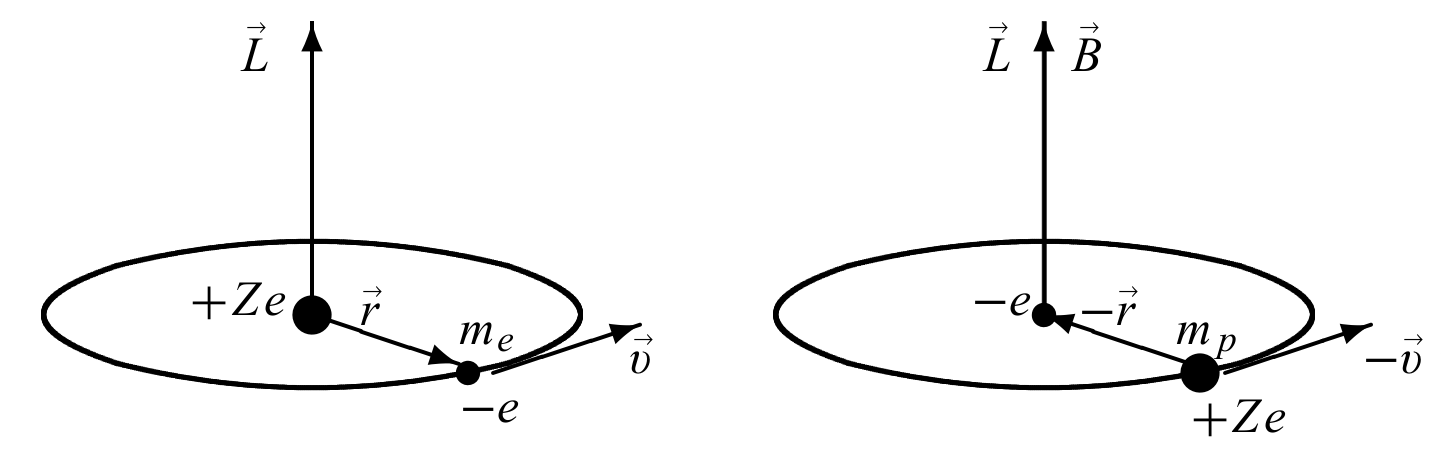
\includegraphics[width=0.8\textwidth]{images/spin-orbit-coupling.png}
    \caption{An electron moving in a circular orbit as seen by the nucleus (left) and the same motion as seen by the electron within its rest frame; the electron sees the nucleus moving in a circular orbit around it (right).}
    \label{fig:spin_orbit_coupling}
\end{figure}

For a more general problem of hydrogen-like atoms (those with one valence electron outside a closed shell) were an electron moves in the (central) Coulomb potential of a nucleus $V(r) = -e\phi(r)$, the electric field is given by:
\begin{equation} \label{eq:electric_field}
    \vec{E}(\vec{r}) = -\nabla\phi(r) = \frac{1}{e}\vec{\nabla} V(r) = \frac{1}{e}\frac{\vec{r}}{r}\frac{dV}{dr}
\end{equation}

So the magnetic field of the nucleus calculated in the rest frame of the electron is obtained by inserting \textbf{Equation \ref{eq:electric_field}} into \textbf{Equation \ref{eq:magnetic_field}}:
\begin{equation}
    \vec{B} = \frac{\vec{E}}{m_ec^2}\times \vec{p} = \frac{1}{em_ec^2}\frac{1}{r}\frac{dV}{dr}\,\vec{r}\times \vec{p} = \frac{1}{em_ec^2}\frac{1}{r}\frac{dV}{dr}\,\vec{L}
\end{equation}

where $\vec{L} = \vec{r}\times \vec{p}$ is the orbital angular momentum of the electron. The interaction of the electron's spin dipole moment $\vec{\mu}_S = -e\vec{S}/m_e$ with the orbital magnetic field $\vec{B}$ of the nucleus gives rise to the following interaction energy:
\begin{equation}
    H_{SO} = -\vec{\mu}_S \cdot \vec{B} = \frac{e}{m_e}\,\vec{S}\cdot \vec{B} = \frac{1}{m_e^2c^2}\frac{1}{r} \frac{dV}{dr}\,\vec{S}\cdot \vec{L}
\end{equation}

This energy turns out to be twice the observed spin-orbit interaction energy. This is due to the fact that $H_{SO}$ was calculated within the rest frame of the electron. This frame is not inertial, for the electron accelerates while moving in a circular orbit around the nucleus. For a correct treatment, we must transform to the rest frame of the nucleus (i.e., the lab frame). This transformation, which involves a relativistic transformation of velocities, gives rise to an additional motion resulting from the precession of $\vec{\mu}_S$; this is known as the \textit{Thomas precession}. The precession of the electron's spin moment is a relativistic effect which occurs even in the absence of an external magnetic field. The transformation back to the rest frame of the nucleus leads to a reduction of the interaction energy computed before by a factor of $2$:
\begin{equation}
    H_{SO} = \frac{1}{2m_e^2c^2}\frac{1}{r} \frac{dV}{dr}\,\vec{S}\cdot \vec{L}
\end{equation}

In order to obtain the quantum mechanical expression from this classically obtained result, one need only replace the classical quantities $\vec{S}$ and $\vec{L}$ by their quantum mechanical operators.

For a hydrogen's electron, $V(r)=-e^2/r$ and $dV/dr=e^2/r^2$, so that:
\begin{equation}
    H_{SO} = \frac{e^2}{2m_e^2c^2}\frac{1}{r^3}\,\vec{S}\cdot \vec{L}
\end{equation}

If we consider only this as a standalone Hamiltonian, we can find the energy eigenvalues by taking $\vec{S}\cdot \vec{L} = \frac{1}{2}(\vec{J}\,^2 - \vec{L}\,^2 - \vec{S}\,^2)$, which comes from expanding $\vec{J}\,^2 = (\vec{L}+\vec{S})^2$:
\begin{equation}
    H_{SO} = \frac{e^2}{4m_e^2c^2}\frac{1}{r^3}(\vec{J}\,^2 - \vec{L}\,^2 - \vec{S}\,^2) \longrightarrow E_{SO} = \frac{\hbar^2}{4m_e^2c^2}\frac{e^2}{r^3}\ (j(j+1)-l(l+1)-s(s+1))
\end{equation}

In terms of the Bohr magneton $\mu_B = e\hbar/2m_e$:
\begin{equation}
    E_{SO} = \frac{\mu_B^2}{c^2r^3} \left[j(j+1)-s(s+1)-l(l+1)\right]
\end{equation}

The scales of energies associated with the spin-orbit coupling are about two orders of magnitude smaller than the energies associated with the discrete atomic levels, so we can consider this energy $H_{SO}$ as a \textit{perturbation} to the Hamiltonian of the hydrogen atom and use \textit{stationary perturbation theory}\footnote{We will discuss this in more detail in the next chapter.} to calculate corrections due to the spin-orbit coupling:
\begin{equation}
    H = H_0 + H_{SO} = \frac{\vec{p}\,^2}{2m_e}-\frac{e^2}{r} + \frac{e^2}{2m_e^2c^2}\frac{1}{r^3}\vec{S}\cdot \vec{L}
\end{equation}

where $H_0$ is the unperturbed Hamiltonian and $H_{SO}$ is the spin-orbit coupling perturbation.

\subsubsection{The Zeeman effect}

As we have discussed in previous sections, the electron posesses both an orbital magnetic dipole moment, $\vec{\mu}_L$, and a spin magnetic dipole moment, $\vec{\mu}_S$. Both of these moments give rise to two energy terms when the electron is submitted to a magnetic field $\vec{B}$, $-\vec{\mu}_L\cdot \vec{B}$ and $-\vec{\mu}_S\cdot \vec{B}$, whose sum we call the Zeeman energy. Using \textbf{Equation \ref{orbital_magnetic_dipole_moment}} and \textbf{Equation \ref{spin_magnetic_dipole_moment}}, we can write the Zeeman energy as\footnote{Here, we have used the fact that $g_s = 2$ and $q=-e$ for the electron.}:
\begin{equation}
    H_Z = -\vec{\mu}_L\cdot \vec{B} - \vec{\mu}_S\cdot \vec{B} = \frac{e}{2m_e}\vec{L}\cdot \vec{B} + \frac{e}{m_e}\vec{S}\cdot \vec{B} = \frac{e}{2m_e}\left(\vec{L}+2\vec{S}\right)\cdot \vec{B}
\end{equation}

We can write this in terms of Bohr's magneton $\mu_B = \frac{e\hbar}{2m_e}$ as:
\begin{equation}
    H_Z = \frac{\mu_B }{\hbar}\left(\vec{L}+2\vec{S}\right)\cdot \vec{B}
\end{equation}

What we have just described is the energy corresponding to the so called \textbf{anomalous Zeeman effect}, which takes into account the spin of the electron. The \textbf{normal Zeeman effect} is the case where we only consider the orbital angular momentum of the electron, which yields the following expression for the energy:
\begin{equation}
    H_Z = \frac{\mu_B}{\hbar}\,\vec{L}\cdot \vec{B}
\end{equation}

\textbf{The normal Zeeman effect}

Let us first consider the normal Zeeman effect. For simplicity, we shall take $\vec{B} = B\vec{e}_z$, so that:
\begin{equation}
    H_z = \frac{\mu_B B}{\hbar}\,L_z
\end{equation}

Solving the eigenvalue equation for the total energy $H = H_0+H_Z$, we find:
\begin{equation}
    \begin{split}
        H\ket{n,l,m_l} &= (H_0+H_Z)\ket{n,l,m_l} = H_0\ket{n,l,m_l} + \frac{\mu_B B}{\hbar}\,L_z\ket{n,l,m_l} = \\
        &= E_n^0\ket{n,l,m_l} + \frac{\mu_B B}{\hbar}\,\hbar m_l\ket{n,l,m_l} = \left( E_n^0 + m_l\mu_B B \right)\ket{n,l,m_l}
    \end{split}
\end{equation}

Therefore, the difference between two consecutive energy levels for each value of $n$ is given by:
\begin{equation}
    \Delta E = \mu_B B
\end{equation}

Take the example of $n=2$, where we have $l = 0, 1$:
\begin{itemize}
    \item When $l=0$, we will only have one value of $m_l$, which is $m_l = 0$. Therefore, we will only have a single energy level:
    \begin{itemize}
        \item[$\to$] $E_{0,0} = E_2^0$
    \end{itemize}
    \item When $l=1$, we will have three possible values of $m_l$, which are $m_l = -1, 0, 1$. Therefore, we will obtain three energy levels:
    \begin{itemize}
        \item[$\to$] $E_{1,-1} = E_2^0 - \mu_B B$
        \item[$\to$] $E_{1,0} = E_2^0$
        \item[$\to$] $E_{1,1} = E_2^0 + \mu_B B$
    \end{itemize}
\end{itemize}

Overall, we have just three \textit{unique} values of the energy. Experimentally, the way we would expect to see this is by observing the splitting of the spectral lines of the atom in the presence of a magnetic field. Instead of seeing \textit{one} line, we would see \textit{three} energy levels: one corresponding to the original level and two at the levels shifted by $\pm \mu_B B$. In general, we would see $2l+1$ lines, corresponding to the $2l+1$ possible values of $m_l$, so that we would always have an odd number of lines in any spectra.


\textbf{The anomalous Zeeman effect}

Unfortunately, in many cases the results of the normal Zeeman effect disagree with the experimental observations. For instance, spectral lines can sometimes split into an \textit{even} number of levels, which could never happen according to the normal Zeeman effect. Why, then, does this happen? The answer, of course, is \textit{spin}. We will now see the two different cases of anomalous Zeeman effect, depending on the strength of the magnetic field $\vec{B}$.

\textit{a) Strong} $\vec{B}$

Let us again consider $\vec{B} = B\vec{e}_z$, so that:
\begin{equation}
    H_Z = \frac{\mu_B B}{\hbar}\left(L_z+2S_z\right)
\end{equation}

In order to find a general result considering spin, it is also important to take into account the spin-orbit coupling effects. Therefore, we need to include the term $H_{SO}$ in our Hamiltonian, so that the eigenvalue equation for the general anomalous Zeeman effect becomes:
\begin{equation}
    \begin{split}
        H\ket{n,l,m_l,m_s} &= (H_0+H_Z)\ket{n,l,m_l,m_s} = \\
        &= H_0\ket{n,l,m_l,m_s}+\frac{\mu_B B}{\hbar}\left(L_z+2S_z\right)\ket{n,l,m_l,m_s} = \\
        &= E_n^0\ket{n,l,m_l,m_s} + \frac{\mu_B B}{\hbar}\left(\hbar m_l+2\hbar m_s\right)\ket{n,l,m_l,m_s} = \\
        &= \left[E_n^0+  (m_l+2m_s)\mu_B B\right] \ket{n,l,m_l,m_s}
    \end{split}
\end{equation}

Therefore, the energy levels $E_n^0$ are shifted by:
\begin{equation}
    \Delta E = (m_l+2m_s)\mu_B B 
\end{equation}

Take the same example as before of $n=2$, where we have $l = 0, 1$. The electron has spin $s=1/2$, so $m_s=\pm 1/2$. Then:
\begin{itemize}
    \item When $l=0$, we will only have one value of $m_l$, which is $m_l = 0$. However, we now have to consider $m_s$, which is has two possible values, $\pm 1/2$. Therefore, we will obtain two different energy levels:
    \begin{itemize}
        \item[$\to$] $E_{0,0,\frac12} = E_2^0 +\mu_B B$
        \item[$\to$] $E_{0,0,-\frac12} = E_2^0 -\mu_B B$
    \end{itemize}
    \item When $l=1$, we will have three possible values of $m_l$, which are $m_l = -1, 0, 1$. For each of the values of $m_l$, we have two possible values of $m_s$, so we will obtain six different energy levels for $l=1$:
    \begin{itemize}
        \item[$\to$] $E_{1,1,\frac12} = E_2^0 + 2\mu_B B$
        \item[$\to$] $E_{1,0,\frac12} = E_2^0 + \mu_B B$
        \item[$\to$] $E_{1,-1,\frac12} = E_2^0$
        \item[$\to$] $E_{1,1,-\frac12} = E_2^0$
        \item[$\to$] $E_{1,0,-\frac12} = E_2^0 - \mu_B B$
        \item[$\to$] $E_{1,-1,-\frac12} = E_2^0 - 2\mu_B B$
    \end{itemize}
\end{itemize}

Overall, we have \textit{five} unique values of the energy, which is two more than what we expected from the normal Zeeman effect. There is still an odd number of energy levels. However, if we computed the energy levels for $n = 1$, we will have only the case $l=0$, which will give the same levels as the $l=0$ case for $n=2$ that we just computed, which were only two. That is, $n=1$ will show an \textit{even} number of energy levels. Both these cases ($n=1$ and $n=2$) are shown in \textbf{Figure \ref{fig:strong_B_zeeman}}.

\begin{figure}[htbp]
    \centering
    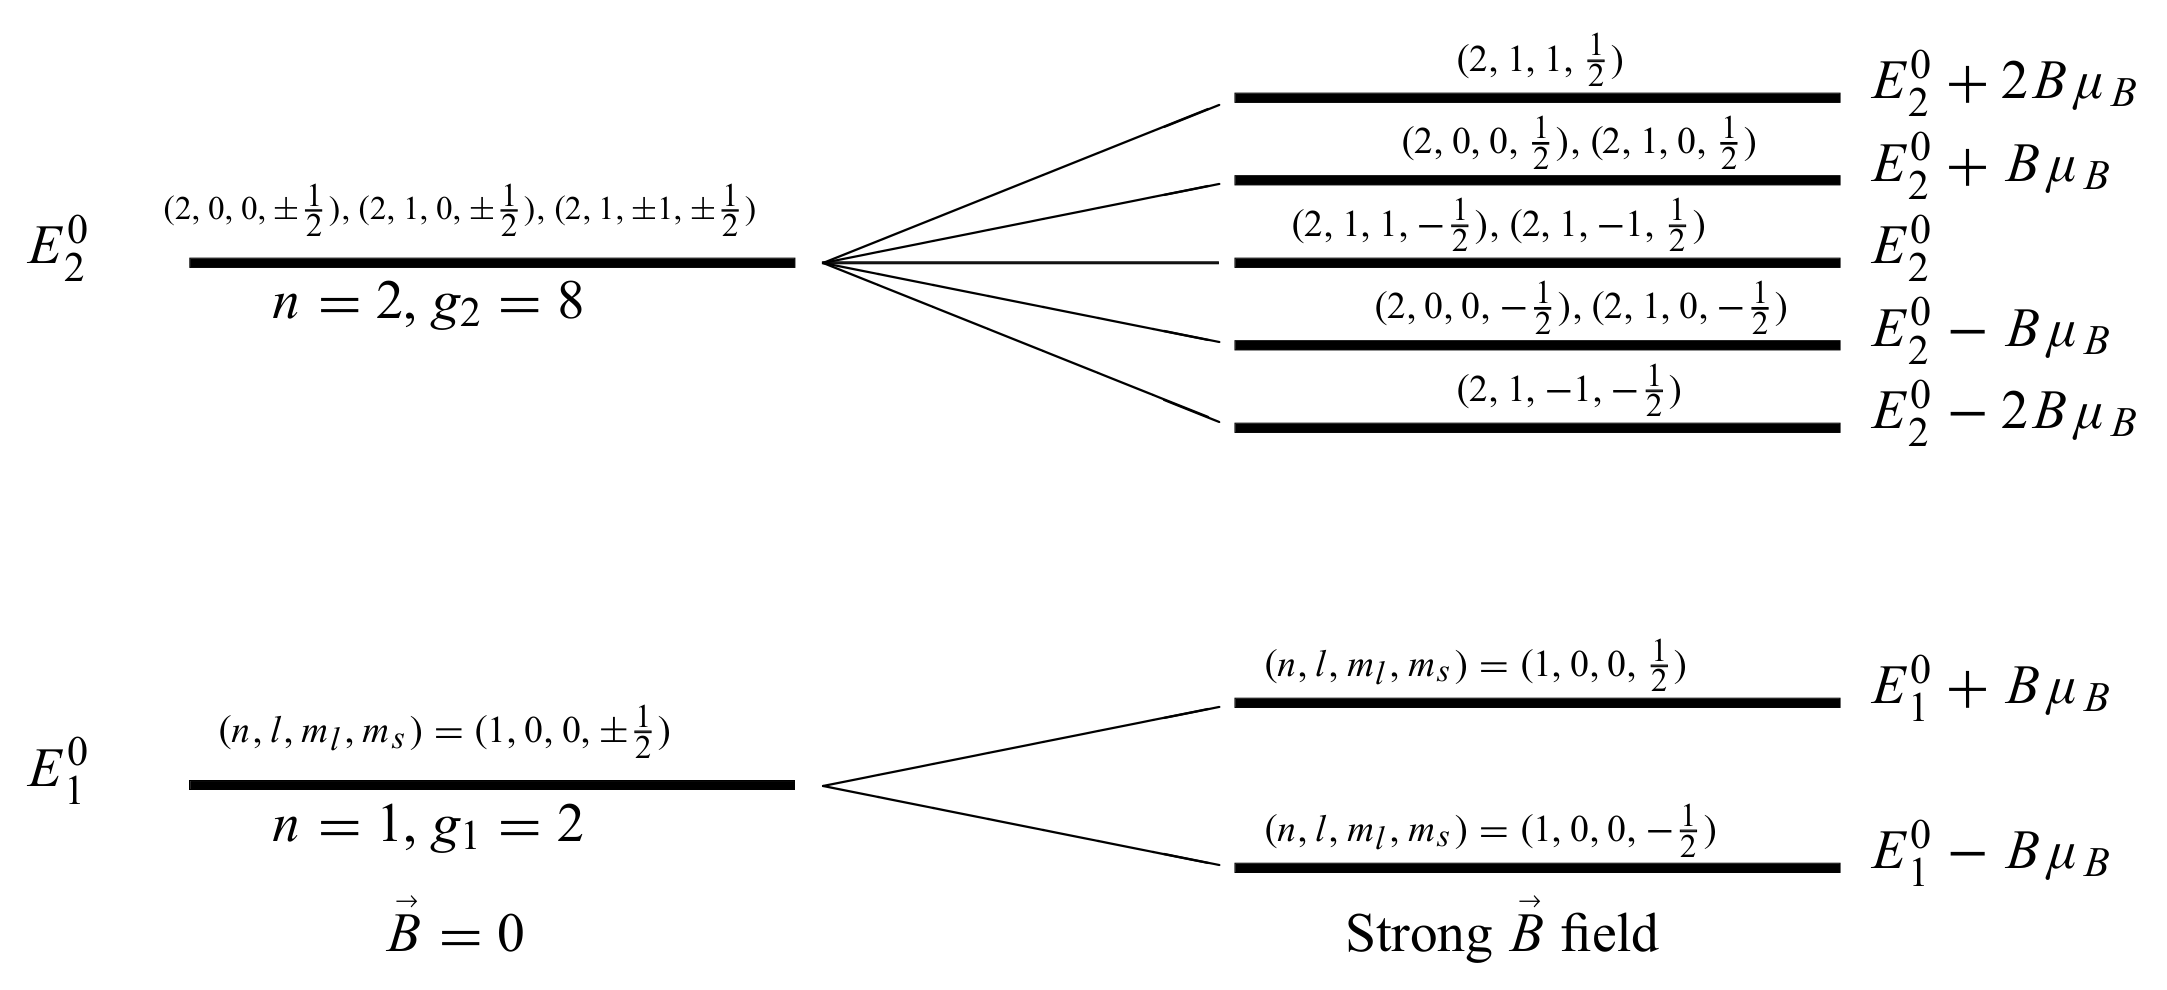
\includegraphics[width=0.8\textwidth]{images/strong_B_zeeman.png}
    \caption{Energy level splitting in the absence of a magnetic field (left) and in the presence of a strong magnetic field $\vec{B}$ (right).}
    \label{fig:strong_B_zeeman}
\end{figure}

\textit{a) Weak} $\vec{B}$

In the case where we have a weak magnetic field $\vec{B}$, we can no longer neglect the spin-orbit coupling effects\footnote{In reality, we should consider not only the spin-orbit coupling, but also the relativistic correction. Both of these together conform the \textit{fine structure} of hydrogen. However, for simplicity, we will only consider the spin-orbit coupling effects in our analysis.}. Then, the best eigenstates to use are $\ket{n,l,j,m_j}$, as they are simultaneous eigenstates of $H_0$ and $H_{SO}$. It is therefore necessary to rewrite $H_Z$ so that $\vec{S}$ and $\vec{L}$ only appear as square operators\footnote{\color{red}Why?}. To do this, let us first consider:
\begin{equation}
    \vec{J} = \vec{S} + \vec{L} \longrightarrow \vec{L} = \vec{J} - \vec{S}
\end{equation}
Then:
\begin{equation}
    \vec{L}\,^2 = \vec{J}\,^2 - \vec{S}\,^2 - \vec{J}\cdot \vec{S} - \vec{S}\cdot \vec{J} \stackrel{\footnotemark}{=}\footnotetext{Remember that, as $\vec{L}$ and $\vec{S}$ commute (they act on different spaces $\varepsilon_{\vec{r}}$ and $\varepsilon_s$), then $\vec{J}$ and $\vec{S}$ also commute: $\vec{J}\cdot\vec{S}-\vec{S}\cdot\vec{J} = (\vec{L} + \vec{S})\cdot \vec{S} - \vec{S}\cdot (\vec{L} + \vec{S}) = \vec{L}\cdot \vec{S} + \vec{S}\,^2 - \vec{S}\cdot\vec{L} - \vec{S}\,^2=0$. } \vec{J}\,^2 - \vec{S}\,^2 -2\vec{J}\cdot \vec{S} \longrightarrow \vec{J}\cdot \vec{S} = \frac{\vec{J}\,^2 - \vec{S}\,^2 - \vec{L}\,^2}{2}
\end{equation}

Therefore:
\begin{equation}
    \begin{split}
        H_Z &= \frac{\mu_B}{\hbar} \left(\vec{L}+ 2\vec{S}\right)\cdot \vec{B} = \frac{\mu_B}{\hbar} \left(\vec{J}+ \vec{S}\right)\cdot \vec{B} = \frac{\mu_B}{\hbar} \left(1+ \frac{\vec{S}}{\vec{J}}\right)\vec{J}\cdot \vec{B} = \\
        &= \frac{\mu_B}{\hbar} \left(1+ \frac{\vec{J}\cdot \vec{S}}{\vec{J}\,^2}\right)\vec{J}\cdot \vec{B} = \frac{\mu_B}{\hbar} \left(1+ \frac{\vec{J}\,^2 - \vec{S}\,^2 - \vec{L}\,^2}{2\vec{J}\,^2}\right)\vec{J}\cdot \vec{B}
    \end{split}
\end{equation}


Then, we write the eigenvalue equation, assuming that $\vec{J}\,||\vec{B}$\footnote{\color{red}We are computing the energy when the electrons are exposed to $\vec{B}$, which causes their spin angular momentum to align with the magnetc field. Why do we assume the whole angular momentum is aligned?}:
\begin{equation}
    \begin{split}
        H\ket{n,l,j,m_j} &= (H_0+H_{SO}+H_Z)\ket{n,l,j,m_j} =\\
        &= E_n^0\ket{n,l,j,m_j} + E_{SO}\ket{n,l,j,m_j} + \frac{\mu_B}{\hbar} \left(1+ \frac{\vec{J}\,^2 - \vec{S}\,^2 - \vec{L}\,^2}{2\vec{J}\,^2}\right)\vec{J}\cdot \vec{B} \ket{n,l,j,m_j} = \\
        &= \left[ E_n^0 + E_{SO} + \frac{\mu_B}{\hbar}\left(1+\frac{j(j+1)-s(s+1)-l(l+1)}{2j(j+1)}\right)\hbar m_jB\right]\ket{n,l,j,m_j}=\\
        &= \left[E_n^0 + E_{SO} + g_jm_j\mu_B B\right]\ket{n,l,j,m_j}
    \end{split}
\end{equation}

Therefore, the energy levels are shifted by two terms: $E_{SO}$, corresponding to spin-orbit coupling and $E_Z = g_jm_j\mu_B B$, corresponding to the Zeeman effect, where $g_j$ is called the Landé factor and is defined as:
\begin{equation}
    g_j = 1 + \frac{j(j+1) - s(s+1)-l(l+1)}{2j(j+1)}
\end{equation}

Recall from the discussion about spin-orbit coupling that:
\begin{equation}
    E_{SO} = \frac{\mu_B^2}{c^2r^3} \left[j(j+1)-s(s+1)-l(l+1)\right]
\end{equation}

Therefore, the effect of the magnetic field on the atom is to split the energy levels first due to the spin-orbit cupling effect, and then to further split those lines due to the Zeeman effect by an amount equal to:
\begin{equation}
    \Delta E_Z = B\mu_B\Delta m_jg_j
\end{equation}

Take the simple example where $n=1$, where we have $l = 0$. The electron has spin $s=1/2$, so $m_s=\pm 1/2$. We also have two different values of $j$, which are $j = l+s = \frac12$ and $j = l - s = -\frac12$. Then\footnote{\color{red}Check all this}:
\begin{itemize}
    \item When $j=\frac12$, we will have a spin-orbit coupling energy of:
    \begin{equation}
        E_{SO,\frac12} = \frac{\mu_B^2}{c^2r^3}\left[\frac12 \left(\frac12+1\right)-\frac12\left(\frac12+1\right)-0\left(0+1\right)\right] = 0
    \end{equation}
    and a Landé factor of:
    \begin{equation}
        g_{j=\frac12} = 1+\frac{\frac12 \left(\frac12+1\right)-\frac12\left(\frac12+1\right)-0\left(0+1\right)}{2\cdot \frac12 \left(\frac12+1\right)} = 1
    \end{equation}
    Therefore, for the two possible values of $m_j$, we will obtain:
    \begin{itemize}
        \item[$\to$] $E_{0,0,\frac12} = E_n^0+\frac{\mu_B B}{2}$
        \item[$\to$] $E_{0,0,-\frac12} = E_n^0-\frac{\mu_B B}{2}$
    \end{itemize}
    \item When $j=-\frac12$, we will have a spin-orbit coupling energy of:
    \begin{equation}
        E_{SO,\frac12} = \frac{\mu_B^2}{c^2r^3}\left[-\frac12 \left(-\frac12+1\right)-\frac12\left(\frac12+1\right)-0\left(0+1\right)\right] = -\frac{\mu_B^2}{c^2r^3}
    \end{equation}
    and a Landé factor of:
    \begin{equation}
        g_{j=\frac12} = 1+\frac{-\frac12 \left(-\frac12+1\right)-\frac12\left(\frac12+1\right)-0\left(0+1\right)}{2\cdot \left(-\frac12\right) \left(-\frac12+1\right)} = 3
    \end{equation}
    Therefore, for the two possible values of $m_j$, we will obtain:
    \begin{itemize}
        \item[$\to$] $E_{0,0,\frac12} = E_n^0 -\frac{\mu_B^2}{c^2r^3}+\frac{3}{2}\mu_B B$
        \item[$\to$] $E_{0,0,-\frac12} = E_n^0-\frac{\mu_B^2}{c^2r^3}-\frac{3}{2}\mu_B B$
    \end{itemize}
\end{itemize}

Overall, just for $n=1$, we have \textit{four} unique values of the energy, due to the spin-orbit coupling effect.